\documentclass[a4paper,12pt]{article}
\usepackage{color}
\usepackage{graphicx, gensymb}
\usepackage{amsfonts, cancel, amssymb}
\usepackage{amsmath, amsthm, array, esvect, esint}
\usepackage{typearea}
\usepackage[a4paper,left=2cm,right=2cm,top=2cm,bottom=3cm,bindingoffset=5mm]{geometry}
\usepackage{tikz} 
\usetikzlibrary{shapes,arrows,positioning,automata,backgrounds,calc,er,patterns}
\usepackage{tikz-feynman}
\tikzfeynmanset{compat=1.0.0}
\newcommand\numberthis{\addtocounter{equation}{1}\tag{\theequation}}
\newcommand{\bra}{}
\newcommand{\kom}{}
\newcommand{\brak}{}
\newcommand{\braket}{}
\newcommand{\intx}{}
\newcommand{\intr}{}
\newcommand{\kla}{}
\newcommand{\klam}{}
\newcommand{\klammer}{}
\newcommand{\oper}{}
\newcommand{\tecxt}{}
\newcommand{\Bra}{}
\newcommand{\Ket}{}

\begin{document}

\title{10 Helizität und Resonanzen}
\author{Joachim Schwardt}
\date{\today}
\maketitle

\section*{Aufgabe 10.2: Helizität vs. Chiralität}
Sei $u_{1,2}=\binom{\chi^+_{1,2}}{\chi^-_{1,2}}$ mit $\chi^\pm_1=\binom{\sqrt{E\pm m}}{0}$ und $\chi^\pm_2=\binom{0}{\pm\sqrt{E\pm m}}$. Für den Operator $P_L:=\frac{1}{2}(1-\gamma^5)$ mit $\gamma^5=\begin{pmatrix}
0&1\\ 1& 0
\end{pmatrix} $ gilt dann:
\begin{align*}
P_Lu_i&=\frac{1}{2}\binom{\chi_i^+-\chi_i^-}{\chi_i^--\chi_i^+}\\
\Rightarrow\ \ \ |P_Lu_i|^2&=\kla\left( {\sqrt{E+m}\mp\sqrt{E-m}} \right)^2=2E\mp 2|\vec{p}|=2m\gamma (1\mp\beta)
\end{align*}
Daraus folgt für rein linkshändige Teilchen die Wahrscheinlichkeit, eine Helizität von $h=\pm\frac{1}{2}$ zu messen:
\begin{align*}
p_+&=\frac{|P_Lu_1|^2}{|P_Lu_1|^2+|P_Lu_2|^2}=\frac{1-\beta}{2}\\
p_-&=\frac{|P_Lu_2|^2}{|P_Lu_1|^2+|P_Lu_2|^2}=\frac{1+\beta}{2}
\end{align*}
Die mittlere Helizität ergibt sich dann zu
\begin{align*}
\bra\langle {h}\rangle&=p_+h_++p_-h_-=\frac{1-\beta}{4}-\frac{1+\beta}{4}=-\frac{\beta}{2}
\end{align*}\,\newpage
\section*{Aufgabe 10.3: Prozesse der schwachen Wechselwirkung}
Die Bosonen der schwachen Wechselwirkung haben einen schwachen Isospin von $T_3(Z,W^\pm)=(0,\pm 1)$. Für linkshändige Fermionen mit der elektrischen Ladung $Q_f$ ist $T_3(f)=\frac{1}{2}\tecxt\text{sign\,}Q_f$, die Neutrinos haben $T_3=\frac{1}{2}$. Die rechtshändigen Antifermionen haben den entgegengesetzten Wert. Die rechtshändigen Fermionen und linkshändigen Antifermionen haben keinen schwachen Isospin. Damit sind folgende Zerfälle möglich:
\begin{align*}
W^+ &\longrightarrow\binom{e^+}{\nu_e},\ \binom{\mu^+}{\nu_\mu},\ \binom{\tau^+}{\nu_\tau}\\
W^- &\longrightarrow\binom{e^-}{\overline{\nu}_e},\ \binom{\mu^-}{\overline{\nu}_\mu},\ \binom{\tau^-}{\overline{\nu}_\tau}
\end{align*}
\begin{figure}[h!]
\centering
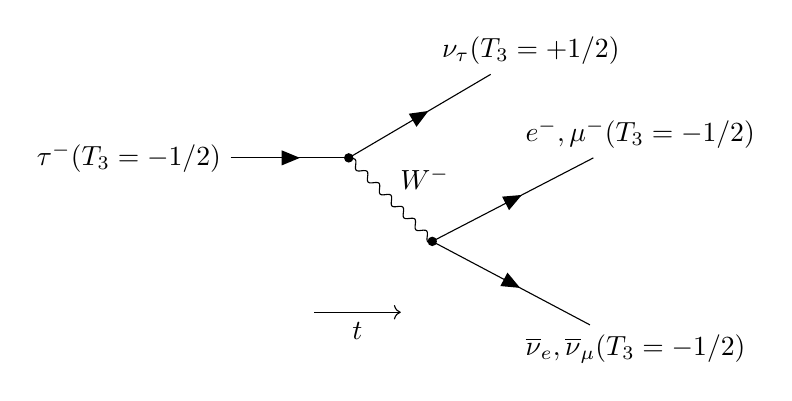
\begin{tikzpicture}
\begin{feynman}
\vertex (a);
\vertex [left =of a] (tau){$\tau^- (T_3=-1/2)$};
\vertex [above right= of a] (nutau){$\nu_\tau (T_3=+1/2)$};
\vertex [below right= of a] (w);
\vertex [above right= of w] (lep){$e^-,\mu^- (T_3=-1/2)$};
\vertex [below right= of w] (nu){$\overline{\nu}_e,\overline{\nu}_\mu (T_3=-1/2)$};
\vertex [below left= 0.9cm and 1.5cm of w] (t1);
\vertex [below left= 0.9cm and 0.4cm of w] (t2);
\diagram*{
(tau) -- [fermion] (a) -- [fermion] (nutau),
(a) -- [boson, edge label=$W^-$, below left] (w) -- [fermion] (nu),
(w) -- [fermion] (lep),
};
\end{feynman}
\draw[->] (t1) -- (t2) node[midway, below] {$t$};
\fill (a) circle (0.06cm);
\fill (w) circle (0.06cm);
\end{tikzpicture}
\caption{t-Kanal}
\end{figure}\,\newpage
\section*{Aufgabe 10.4: Neutrinooszillationen für zwei Generationen}
Die Masseneigenzustände seien $\Ket | {\nu_i} \rangle=\Ket | {\nu_i(0)} \rangle e^{i(\vec{p}_i\cdot\vec{r}-E_it)}$. Die schwachen Eigenzustände ergeben sich dann durch Linearkombinationen zu $\Ket | {\nu_\alpha} \rangle=U_{\alpha i}\Ket | {\nu_i} \rangle$. Dabei ist $U=\begin{pmatrix}
\cos\theta &\sin\theta \\ -\sin\theta &\cos\theta
\end{pmatrix} $ die orthogonale Mischungsmatrix. Die Zeitentwicklung eines Zustands mit der Anfangsbedingung $\Ket | {\nu(0)} \rangle:=\Ket | {\nu_e} \rangle$ ergibt sich dann mit $\Ket | {\nu_i(0)} \rangle=U_{\alpha i}^\top\Ket | {\nu_\alpha(0)} \rangle$ wie folgt:
\begin{align*}
\Ket | {\nu} \rangle&=\cos\theta e^{i(\vec{p}_1\cdot\vec{r}-E_1t)}\Ket | {\nu_1(0)} \rangle+ \sin\theta e^{i(\vec{p}_2\cdot\vec{r}-E_2t)}\Ket | {\nu_2(0)} \rangle=\\
&=\cos\theta e^{i(p_1x-E_1t)}\kla\left( {\cos\theta\Ket | {\nu_e} \rangle-\sin\theta\Ket | {\nu_\mu } \rangle} \right)+ \sin\theta e^{i(p_2x-E_2t)}\kla\left( {\sin\theta\Ket | {\nu_e} \rangle+\cos\theta\Ket | {\nu_\mu } \rangle} \right)=\\
&=e^{i\phi_1}\klam\left[ {\kla\left( {\cos^2\theta + e^{i(\phi_2-\phi_1)}\sin^2\theta} \right)\Ket | {\nu_e} \rangle+\sin\theta\cos\theta\kla\left( {e^{i(\phi_2-\phi_1)}-1} \right)\Ket | {\nu_\mu } \rangle} \right]
\end{align*}
Dabei ist $\phi_i:=p_ix-E_it$. Setze zudem $\Delta\phi:=\phi_2-\phi_1$. Unter der Annahme $p_1=p_2\equiv p$ und $m\ll p$ vereinfacht sich die Phasendifferenz zu
\begin{align*}
\Delta\phi &=(E_1-E_2)t=p\kla\left( {\sqrt{1+\frac{m_1^2}{p^2}}-\sqrt{1+\frac{m_2^2}{p^2}}} \right)t \simeq \frac{m_1^2-m_2^2}{2p}t
\end{align*}
Betrachte in dieser Näherung die Übergangswahrscheinlichkeit bei der zurückgelegten Strecke $L$:
\begin{align*}
P_{e\mu}&:=|\brak\langle {\nu_\mu}| {\nu(x=L)}\rangle|^2=\left\vert\kla\left( {e^{i\Delta\phi}-1} \right)\sin\theta\cos\theta\right\vert^2=\\
&=\sin^2\theta\cos^2\theta\left\vert\frac{e^{i\Delta\phi/2}-e^{-i\Delta\phi/2}}{2i}\right\vert=\sin^22\theta\sin^2\frac{m_1^2-m_2^2}{4E}L\\
P_{ee}&=1-P_{e\mu}
\end{align*}

\end{document}